\documentclass[12pt]{article}
\usepackage{hyperref}
\usepackage{graphicx}
\usepackage[font=small,labelfont=bf]{caption}
\title{Progetto di fine corso}
\date{17/05/2016}
\author{Alessio Luca,Carlo Sindico}

\begin{document}
	\pagenumbering{arabic}
	
	\begin{titlepage}
		\newcommand{\HRule}{\rule{\linewidth}{0.5mm}}%linea orizzontale
		\center
		
		\textsc{\LARGE Universit\`a degli Studi di Padova}\\[1.5cm] 
		\textsc{\Large Laurea in Informatica}\\[0.5cm]
		\textsc{\large Corso di Tecnologie Web}\\[0.5cm]
		\textsc{\large Progetto di fine corso}\\[0.5cm]
		
		%----------------------------------------------------------------------------------------
		%	TITLE SECTION
		%----------------------------------------------------------------------------------------
		
		\HRule \\[0.4cm]
		{ \huge  2FORCHETTE}\\[0.3cm] 
		\HRule \\[0.4cm]
		
		
		%----------------------------------------------------------------------------------------
		%	AUTHOR SECTION
		%----------------------------------------------------------------------------------------
		
		\begin{minipage}{0.3\textwidth}
			\begin{flushleft} \large
				\emph{Studente:}\\
				Luca \textsc{Alessio} % Your name
			\end{flushleft}
		\end{minipage}
		~
		\begin{minipage}{0.3\textwidth}
			\begin{flushright} \large
				\emph{Matricola:} \\
				\textsc{1070690} % Supervisor's Name
			\end{flushright}
		\end{minipage}\\[2cm]
		
			\begin{minipage}{0.3\textwidth}
				\begin{flushleft} \large
					\emph{Studente:}\\
					Carlo \textsc{Sindico} % Your name
				\end{flushleft}
			\end{minipage}
			~
			\begin{minipage}{0.3\textwidth}
				\begin{flushright} \large
					\emph{Matricola:} \\
					\textsc{1069322} % Supervisor's Name
				\end{flushright}
			\end{minipage}\\[2cm]
			
		%----------------------------------------------------------------------------------------
		%	INFORMATION WEBSITE
		%----------------------------------------------------------------------------------------
		
		\textsc{\Large Informazioni sul sito:}\\[0.3cm]	
		\textit{//tecnologie-web.studenti.math.unipd.it/tecweb/$\sim$csindico/}\\[1cm]
		
		%----------------------------------------------------------------------------------------
		%	DATI LOGIN
		%----------------------------------------------------------------------------------------
		
			\textsc{\Large Login Admin:}\\[0.3cm]
			\textsc{ Username:}\textit{ admin }\\[0.1mm]
			\textsc{ Password:}\textit{ admin }\\[0.1mm]
			
		\vfill
	\end{titlepage}
	
	\newpage
	\renewcommand{\contentsname}{Indice}
	\tableofcontents
	
	
	\newpage
	\pagenumbering{arabic}
	
	\section{Abstract}
	\begin{itemize}
		\item 2Forchette.it \`e un sito dedicato alla raccolta di ricette culinarie. 
		\item L'utenza che accede al sito ha la possibilit\`a di visualizzare le ricette attualmente presenti ed eventualmente di proporne di nuove. Le ricette vengono suddivise in diverse categorie per facilitarne la consultazione e contengono dettagliate informazioni sulla loro preparazione.

		\item Per ogni ricetta vengono indicati una breve descrizione, la lista degli ingredienti, un'immagine rappresentativa, una spiegazione dettagliata del procedimento da seguire ed altri dati minori (quali tempo di preparazione, difficoltà, autore e numero di persone).

		\item La principale feature del sito \`e costituita dalla sezione "Proponi ricetta", dove appunto l'utente ha la possibilit\`a di inserire una propria ricetta che verr\`a in seguito valutata dall'amministratore ed eventualmente ammessa nel sito.

		\item All'interno del sito l'utente ha inoltre le possibilit\`a di ricercare ricette per nome (funzionalit\`a disponibile in tutte le pagine tramite la barra di ricerca sull' header) e di lasciare eventuali commenti sul sito nella pagina dei contatti.

		\item Si \`e scelto di rendere la navigazione del sito più immediata possibile, ogni ricetta può essere infatti raggiunta con un massimo di 3 click (home $\Rightarrow$ categoria $\Rightarrow$ ricetta, ricerca $\Rightarrow$ ricetta) e il design del sito è minimale e responsive per garantire la massima usabilit\`a.


		\item Per quanto riguarda la parte amministrativa, l'admin pu\`o accedere alla propria console dal link posto nel footer della home (login: admin password: admin), da questa area riservata sar\`a possibile la gestione delle ricette proposte dagli utenti (deciderne quindi l'accettazione o il rifiuto) e l'eventuale eliminazione di ricette ritenute obsolete o di commenti offensivi. Queste funzionalit\`a sono presentate in modo semplice e correlate da una breve spiegazione.
	\end{itemize}


		\section{Utenti destinatari}
		\begin{itemize}
			\item Il target di riferimento di questo sito \`e molto ampio, un sito di cucina viene visitato solitamente da persone appartenenti a varie fasce d'et\`a e con differenti bagagli culturali perci\`o \`e stato scelto di rendere il sito il più semplice ed intuitivo possibile, in particolare \`e stata posta molta attenzione all'accessibilità per utenti non vedenti (ma questo verr\`a approfondito in una sezione apposita). 

		\end{itemize}
		
			\section{Materiale consegnato}
			
			 I file consegnati sono organizzati su 3 cartelle:
			\begin{itemize}
				\item cgi-bin: cartella nella quale sono presenti i file .cgi
				\item data: in questa cartella sono contenuti i file xml ed i relativi XMLSchema.
				\item public-html: contiene index.html e le sotto-cartelle:
\begin{itemize}
\item css: cartella contenente i file .css;
		\item		 images: cartella contenente tutte le foto del sito;
			\item	 js: cartella contenente i vari script realizzati in JavaScript.
\end{itemize}				 
			\end{itemize}	Andiamo ora ad esaminare nel dettaglio le applicazioni di ciascuna tecnologia impiegata nel sito e le loro interazioni. 
			\newpage
			\section{HTML}

 La struttura HTML del sito viene interamente "stampata" da vari file .cgi: questa scelta \`e dovuta alla grande presenza di contenuto dinamico all'interno del sito per cui non sono presenti file .html "puri" se non index.html che \`e per\`o un semplice redirect a menu.cgi, file Perl che effettivamente stampa la homepage. \\ \\
Le pagine HTML del sito (stampate dal cgi) sono state realizzate rispettando lo standard XHTML 1.0 Strict.

			\section{Perl}
			
				  Le pagine scritte in Perl si dividono principalmente in due tipologie: pagine "dinamiche" di rappresentazione e pagine di elaborazione dei dati.\\ \\
				Alla prima tipologia appartengono i file .cgi che eseguono il "print" della pagina html con il contenuto richiesto (ne \`e un esempio la pagina page\_template.cgi che si occupa della stampa a video di ogni ricetta) mentre le pagine della seconda tipologia sono solitamente "pagine di servizio" ovvero codice che esegue operazioni dietro le quinte come salvataggi ed eliminazioni di dati sui file xml. \\ \\Nel dettaglio, questo \`e ci\`o di cui ciascun file si occupa:
\begin{itemize}

				\item  menu.cgi - pagina principale del sito, contiene del contenuto dinamico in quanto le "ricette consigliate" che compaiono nella pagina sono casuali e variano ad ogni accesso alla pagina (inoltre in ogni pagina del sito il footer varia leggermente a seconda se l'amministratore sia loggato oppure meno).
				
				\item  antipasti.cgi, secondi.cgi, primo.cgi, dessert.cgi - semplici sottomen\`u interni che si occupano di raggruppare le ricette appartenenti alla stessa categoria per facilitare la navigazione dell'utente

				\item page\_template.cgi - pagina dinamica che visualizza la ricetta richiesta, funziona nel seguente modo: il link cliccato dall'utente che lo indirizza a questa pagina contiene un parametro (id) differente per ogni ricetta, page\_template.cgi cerca il parametro passato tra gli attributi IDCode delle singole ricette nel file 4forchette.xml (vedi sezione XML) ed identifica quale era la ricetta richiesta di cui va poi a restituirne le informazioni su schermo.

				\item proponiricetta.cgi - stampa la pagina "Proponi una ricetta" attraverso la quale l'utente ha la possibilit\`a di proporre nuove ricette da inserire nel sito. La pagina contiene un form di discrete dimensioni e delle istruzioni sul suo completamento. Un'analisi pi\`u dettagliata su come avviene il processo di creazione, memorizzazione e approvazione delle ricette verr\`a effettuata in un successivo paragrafo.

				\item handle\_proposta.cgi - quando l'utente ha compilato correttamente (vedi sezione Javascript) il form per la proposta di una nuova ricetta, la ricetta viene salvata nel "database" xml. La nuova ricetta non verr\`a tuttavia ancora visualizzata nel sito, prima dovr\`a infatti venire approvata dall'amministratore (vedi accept\_ricetta.cgi).

				\item contatti.cgi - stampa la pagina dei contatti, qui l'utente ha la possibilità di vedere i messaggi lasciati da altri utenti ed eventualmente pu\`o lasciarne uno proprio compilando il form apposito dove viene richiesto un nome ed il testo effettivo del commento (sarebbe stato interessante implementare un sistema di registrazione e gestione degli utenti nel sito ma date le scarse dimensioni del gruppo e il tempo disponibile si \`e optato per una soluzione meno impegnativa).

				\item inserisci\_commento.cgi - gestisce l'inserimento di un nuovo commento traducendo l'input dell'utente in dati xml.

				\item amministratore\_login.cgi - contiene il form che l'amministratore utilizza per effettuare l'accesso all'area riservata. Questa pagina \`e accessibile solamente dal link posto nel footer della pagina principale (menu.cgi).

				\item controllo\_login.cgi - controlla la correttezza delle credenziali inserite nel form del punto precedente. Al momento \`e previsto un solo amministratore per il sistema. L'amministratore viene identificato come autenticato quando un parametro apposito (\$auth) \`e impostato ad un preciso valore e ci\`o viene settato in degli appositi cookie (vedi codice del file per i dettagli) per rendere l'informazione nota tra le diverse pagine.

				\item console\_admin.cgi - stampa l'hub amministrativo da cui \'e possibile gestire semplicemente l'intero sito. Da questa pagina l'amministratore ha la possibilit\`a di accettare o rifiutare le nuove ricette, eliminare vecchie ricette ed eliminare eventuali commenti ritenuti offensivi.

				\item accept\_ricetta.cgi - concede ad una ricetta il permesso di venire visualizzata nel sito (semplicemente il suo attributo accepted viene settato positivamente).

				\item delete\_ricetta.cgi - elimina una ricetta dal file xml. Operazione irreversibile.

				\item delete\_commento.cgi - elimina un commento dal file xml. Operazione irreversibile.

				\item logout.cgi - breve script che effettua il logout dell'amministratore. Viene invocato alla pressione del tasto "logout" visibile sul footer di ogni pagina qualora l'amministratore sia attualmente autenticato nel sistema.

				\item cercaricetta.cgi - nell'header di ogni pagina è presente una barra di ricerca, qualora l'utente digitasse una stringa di caratteri e ne richiedesse l'elaborazione, questo \`e lo script che verrebbe eseguito: cercaricetta.cgi stampa una pagina contente un elenco di tutte le ricette il cui titolo matcha in parte o totalmente il parametro di ricerca inserito dall'utente. La ricerca avviene semplicemente scorrendo l'xml isolandone nomi ed id di tutte le ricette e restituendo solamente quelle che contengono una corrispondenza.

				\item funzioni.pl  contiene funzioni di servizio usate in diversi contesti (ad es. trim degli input).	

\end{itemize}	
			
		\newpage	
	
				
		\section{XML}
		Sono presenti 3 file xml principali con i rispettivi xsd:

		\begin{itemize}
		\item  amministratore.xml - semplice file ausiliario per il controllo del corretto login nell'area amministrativa, contiene solamente due campi per il login e la password.
		
		\item commenti.xml - contiene i commenti contenuti nella sezione contatti; dalla console amministrativa è possibile intervenire indirettamente sul file attuando operazioni di eliminazione
		
		\item 4forchette.xml - cuore centrale del sistema, questo documento xml svolge la funzione di database per le ricette: anche qui l'amministratore può effettuare operazioni di eliminazione mentre l'inserimento è riservato all'utente (questo aspetto \`e esaminato nel dettaglio nelle sezioni successive)
		\end{itemize}				
					
			\section{Javascript}
			\begin{itemize}
				

				\item Javascript \'e stato utilizzato principalmente per il controllo degli input dei form. 
				\item Nel sito sono presenti 3 differenti form, quello per il login nell'area amministrativa, un secondo per il submit dei commenti nella pagina dei contatti ed infine il pi\`u complesso nella sezione per la proposta di nuove ricette. 
				\item Per quanto riguarda i primi due form (gestiti rispettivamente dai file controllo\_login.js e valida\_commento.js), una volta che l'utente clicca su "Submit" vengono analizzati in ordine di apparizione tutti i campi del form, se ne viene identificato uno vuoto allora l'invio viene bloccato e l'utente ne viene notificato da un messaggio d'errore specifico per quel campo.
				\item Per quanto riguarda il form "Proponi ricetta" invece (gestito dal file proponi\_ricetta.js), oltre a questi controlli basilari ne viene effettuato un altro pi\`u approfondito nell'area di inserimento degli ingredienti. 
				\item Dato che ogni ricetta presenta un numero di ingredienti sempre differente era impossibile prevedere un numero definito di campi per ciascun ingrediente nel form (in quanto sarebbero stati spesso insufficienti oppure troppo numerosi e comunque sgradevoli visivamente), per risolvere questo problema si \`e inizialmente pensato di realizzare un form dinamico che aggiungesse campi su richiesta dell'utente. Questa soluzione \`e stata però scartata per difficolt\`a tecniche nella realizzazione e principalmente per il fatto che non fosse accessibile agli screen reader. 
				\item Si \`e optato quindi per lasciare la zona di inserimento degli ingredienti come una semplice area di testo all'interno della quale per\`o vengono applicate delle regole per l'identificazione dei singoli ingredienti: dopo ogni ingrediente \`e necessario inserire il carattere di separazione ";" (punto e virgola senza virgolette) ed andare a capo. Se il testo inserito dall'utente rispetta questa sintassi l'input verr\`a accettato, altrimenti verr\`a fornito un messaggio d'errore. Nella pagina sono presenti delle istruzioni sull'utilizzo del form che spiegano anche l'appropriato inserimento degli ingredienti; riteniamo che la maggior parte degli utenti non trovi difficolt\`a ad usare questa sintassi che \`e inoltre pienamente accessibile ed utilizzabile da utenti non vedenti.		
		
			\end{itemize}
	\newpage
	Come interagiscono le varie tecnologie tra di loro? Vediamo un esempio...
	\section{Step by step: ciclo di vita di una ricetta}
			
\begin{enumerate}
\item L'utente \`e intenzionato a proporre una nuova ricetta e si reca sulla pagina apposita che viene visualizzata dal file proponiricetta.cgi
\item L'utente ha terminato di compilare i campi e preme su "Submit"
\item Viene eseguito lo script proponi\_ricetta.js che controlla prima di tutto se non ci sono campi vuoti e secondariamente se la sintassi del campo "Ingredienti" \`e corretta: se entrambe le condizioni sono soddisfatte si passa al punto successivo, altrimenti si ritorna al punto 2
\item Arrivati a questo punto siamo certi della correttezza dell'input che viene succesivamente processato dal file handle\_proposta.cgi e memorizzato in 4forchette.xml rispettando i criteri stabiliti. In questo momento l'attributo accepted della nuova ricetta \`e impostato a 0 (che simboleggia lo stato di attesa, per cui la ricetta non verr\`a visualizzata all'interno del sito)
\item Al suo successivo accesso nell'area amministrativa, l'admin vedr\`a comparire la nuova ricetta proposta dall'utente nella sezione "Ricette proposte" da dove potr\`a  vederne un'anteprima e di conseguenza decidere se accettarla o meno tramite gli appositi pulsanti
\item Se la ricetta \`e stata scartata essa verr\`a semplicemente eliminata dall'xml, se invece \`e stata accettata il suo attributo accepted verr\`a settato ad 1 (che simboleggia lo stato di accettamento) e la ricetta diverr\`a visibile all'utenza del sito.
\item In qualsiasi momento l'amministratore ha la possibilità di eliminare le ricette, attenzione per\`o che l'eliminazione \`e un' operazione irreversibile!
\end{enumerate}
\newpage
\section{CSS}
			\begin{itemize}
				\item Nella realizzazione dell'interfaccia grafica del sito è stato usato lo standard CSS3.
				\item Allo stesso tempo si \'e fatta molta attenzione alla compatibilit\'a con browser pi\'u datati, e si \'e cercato di utilizzare un numero ristretto delle nuove funzionalit\'a offerte dallo standard.
				
				\item Alcune delle funzionalit\'a CSS3 che sono state utilizzate:
				Border-radius e Box shadow: per realizzare i pulsanti delle form , e per le immagini.
				
			
				\item Nella cartella public-html/css sono presenti i seguenti fogli di stile:

				\subitem style.css: modella lo stile di visualizzazione del sito sia per gli utenti desktop (che hanno uno schermo largo al massimo 1200px) che per gli utenti mobile con dispositivi con schermo piccolo (che hanno uno schermo largo massimo 390px) e dispositivi con dimensioni schermo intermedie ( max-width=730px).


				\subitem print.css: modella lo stile di stampa delle pagine del sito.(particolare attenzione si \'e data alla stampa delle pagine delle ricette).


					Di seguito sono riportate le rispettive visualizzazioni del sito   della versione mobile e desktop:



			\begin{figure}[ht!]
			\centering
			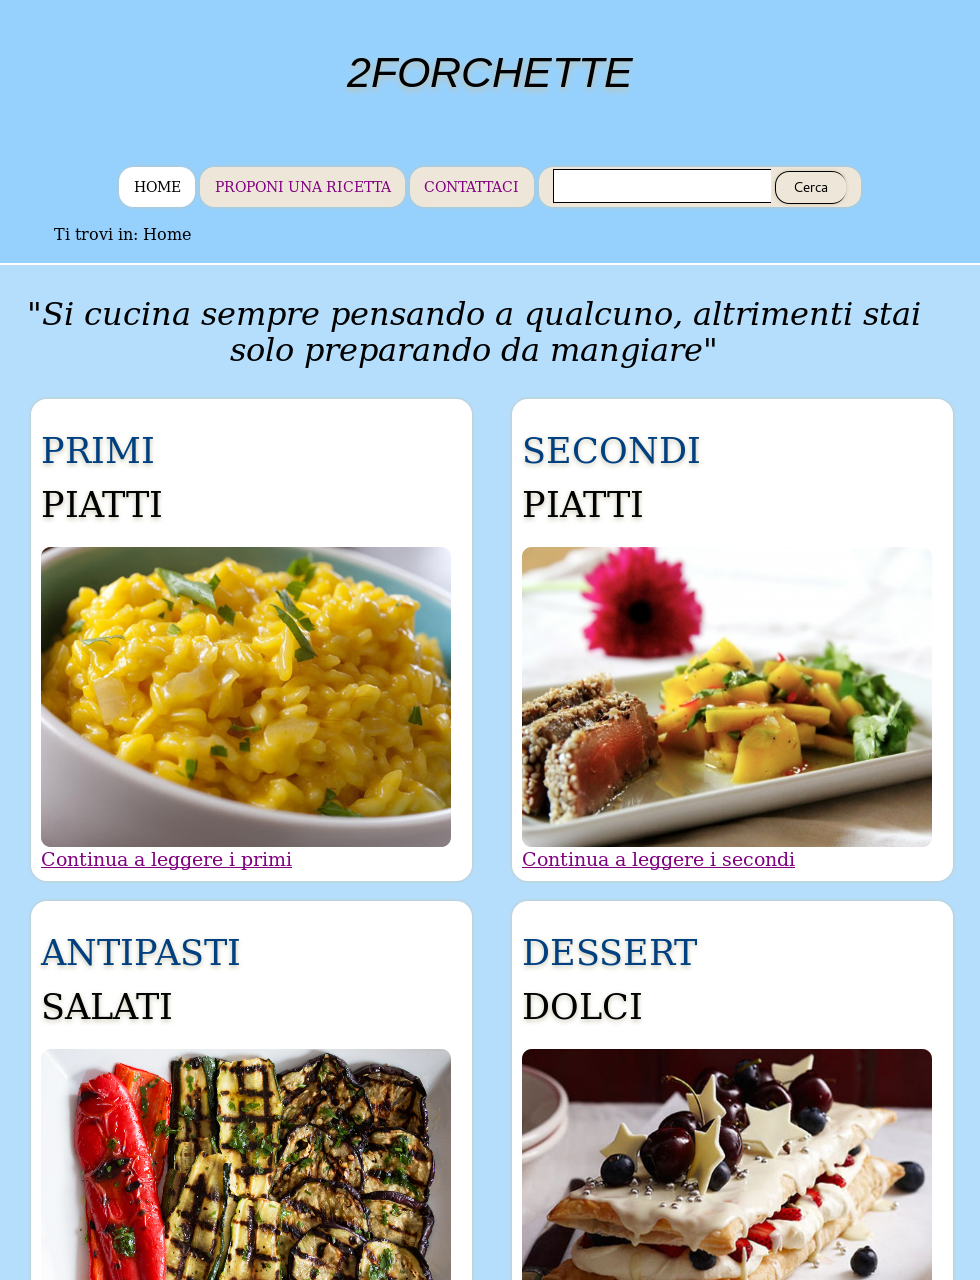
\includegraphics[width=90mm]{desktop}
			\caption{vedi file desktop.png}
			\end{figure}

			\begin{figure}[ht!]
			\centering
			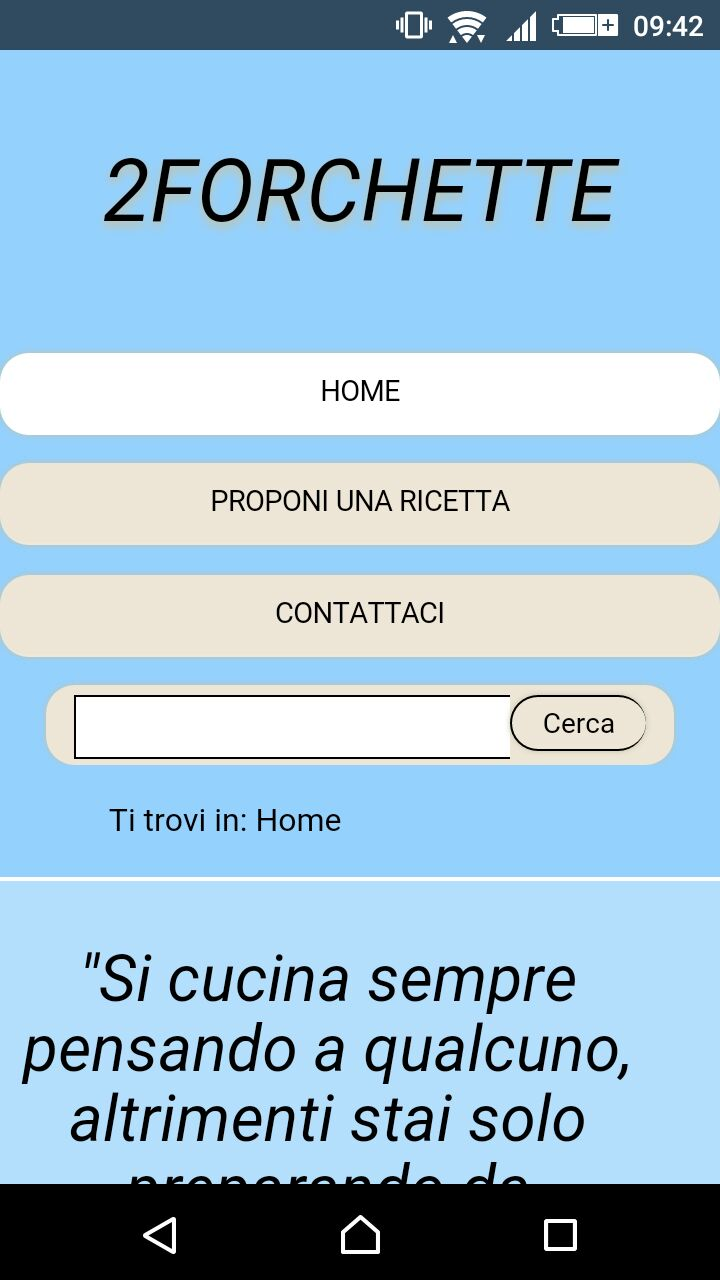
\includegraphics[width=90mm]{mobile}
			\caption{vedi file mobile.png}
			\end{figure}
		
				\end{itemize}
	

	\newpage
		\section{Accessibilit\`a}
		\subsection{Separazione tra struttura,presentazione e comportamento}
		\begin{itemize}
			\item Per una maggiore accessibilit\'a al sito da parte di utenti disabili e per favorire gli algoritmi dei motori di ricerca si \'e deciso di separarare la struttura dalla presentazione e dal comportamento.
			Infatti il contenuto del sito \'e rapprentato dai file HTML e CGI, i quali richiamano i fogli di stile CSS e si utilizzano (anche in questo caso attraverso percorsi esterni),controlli in JavaScript in particolare per la compilazione dei form. 

			\item Il contenuto rimane accessibile anche se JavaScript \'e disabilitato. Infatti opportuni controlli in Perl ne verificano la validit\`a.

			\item Tutto il codice \'e stato scritto seguendo le disposizioni W3C con opportuna validazione sui loro validatori.
		\end{itemize}
			\subsection{Colori}
			\begin{itemize}
				\item Si \'e scelto uno schema di colori non particolarmente vivace (un mix di azzuri chiaro); anche se non sono colori di base comunque la lettura dei testi risulta accessibile. Per un sito di cucina inoltre è opportuno non utilizzare colori troppi aggressivi e decisi ma attenersi ad uno stile più sobrio e rilassato. 

				\item I link sono sempre sottolineati, e diventano di colore viola quando vengono cliccati.

			Di seguito sono riportate le visualizzazioni del sito attraverso alcuni disturbi visivi:

			\begin{figure}[ht!]
			\centering
			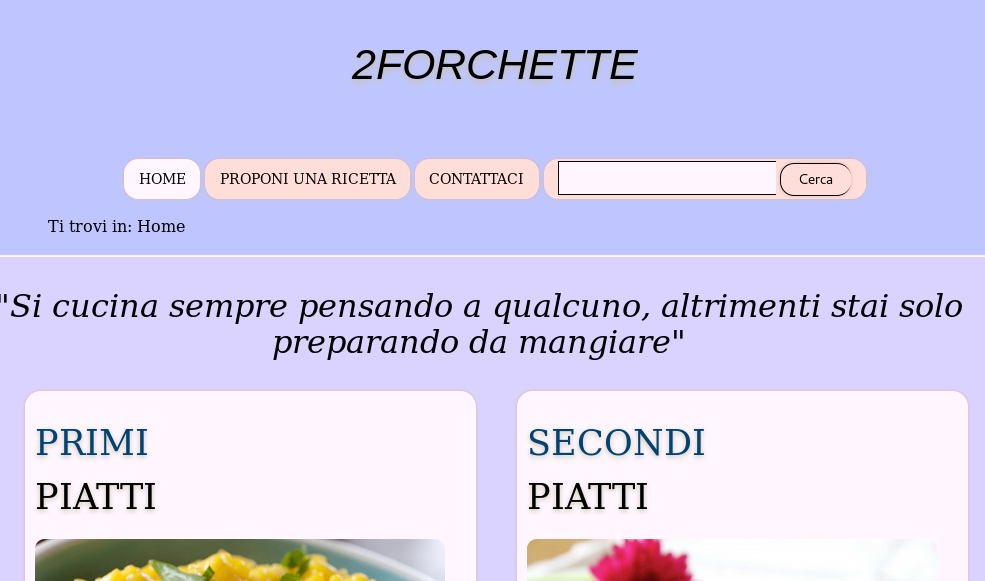
\includegraphics[width=90mm]{deuteranopia}
			\caption{vedi file deuteranopia.png}
			\end{figure} 

			\begin{figure}[ht!]
			\centering
			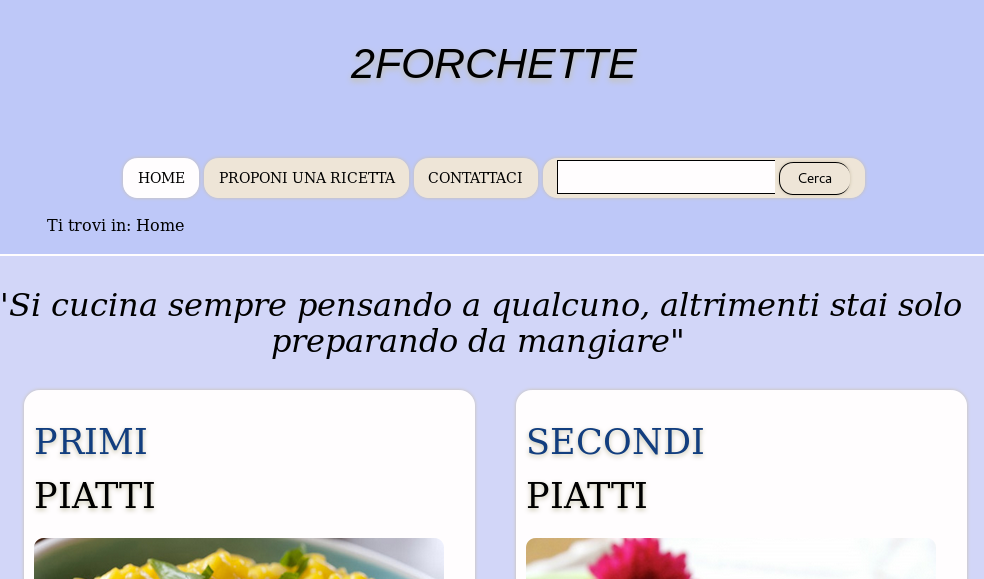
\includegraphics[width=90mm]{protanopia}
			\caption{vedi file protanopia.png}
			\end{figure}

			\begin{figure}[ht!]
			\centering
			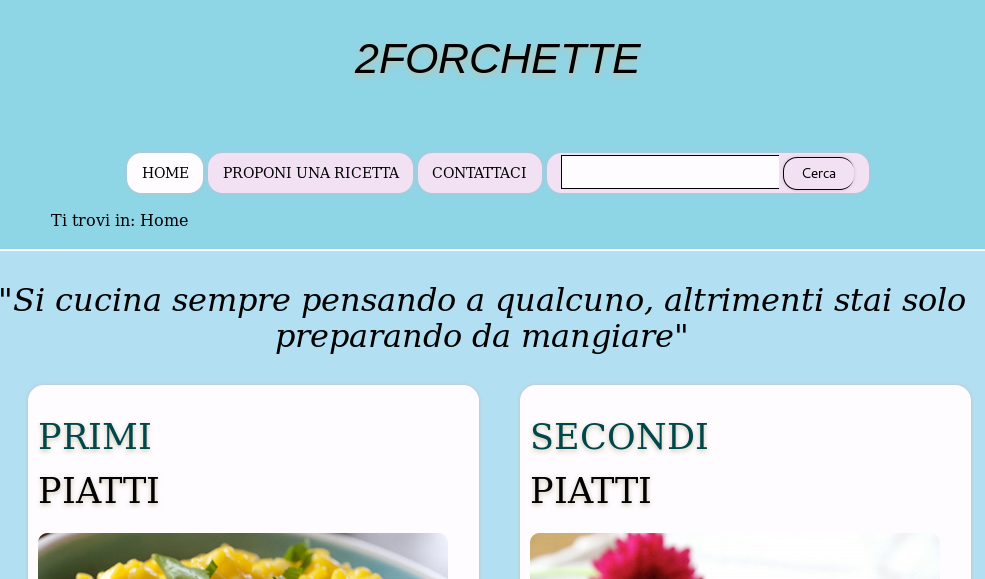
\includegraphics[width=90mm]{tritanopia}
			\caption{vedi file tritanopia.png}
			\end{figure}
			
			\end{itemize}	

			
			\newpage
			\subsection{Tag meta}
			
	 Sono stati inseriti per ogni pagina i tag meta:
	 		\begin{itemize}
				\item title: descrive la pagina corrente dal particolare al generale.
				\item description: da una descrizione del contenuto del sito
				\item keywords: contiene parole chiave per i motori di ricerca
				\item language: indica che il sito \'e stato interamente scritto in italiano.
				\item author: indica l'autore/i del sito
				\item content-type: contiene direttive per il browser
				\item viewport: esprime indicazioni per la visualizzazione
			\end{itemize}
			\subsection{Screen reader}
			\begin{itemize}
				\item Ogni foto ha il suo attributo alt che descrive ci\'o che l'immagine ritrae.
				Si \`e evitato di utilizzare immagini per visualizzare il testo, quindi il contenuto informativo rimane accessibile anche quando fallisce il caricamento delle immagini o del CSS.
				\item Si \'e fornita particolare attenzione alle parole straniere che sono state segnalate agli screenreader attraverso il tag "span xml:lang=en" segnalando la lingua con cui leggere correttamente i vocaboli. 
				\item Inoltre \`e stato inserito un link skip nav per saltare direttamente al contenuto qualora l'utente dello screen reader non voglia riascoltare nuovamente il men\`u
			\end{itemize}
			\section{Usabilit\`a}
			L'utente riesce ad orientarsi nel sito? Analizziamo alcuni degli assi principali del giornalismo. Ometteremo gli assi Who e When dato che nel nostro contesto non \`e necessario dare all'utente informazioni su chi c'\`e dietro al sito (\`e un progetto didattico) n\`e sono presenti novità continue.
			\begin{itemize}
				
				\item What?: 
				Un utente appena entra nella home capisce subito che si tratta di un sito di ricette, dalla barra dei men\'u (Proponi ricetta, Cerca ricetta), e dal contenuto in primo piano che mette in evidenza alcune ricette proposte.
				
				\item Where?: 
				L'utente riesce sempre a capire dove si trova grazie al breadcrumb, inoltre l'header costituisce un importante punto di riferimento per la navigazione dell'utente.
				
				\item Why?: 
				Perch\'e un utente dovrebbe rimanere nel sito o dovrebbe ritornarci? Il sito \'e principalmente espositivo,(gli utenti possono liberamente visualizzare le ricette), si \'e cercato di renderlo pi\'u interessante, aggiungendo una sezione proponi ricetta (l'utente ha la possibilit\'a di inserire la propria ricetta), e anche una sezione commenti.
				
				\item How?:
				 La barra di navigazione mostra tutte le sezioni principali del sito alle quali un utente pu\'o accedere.
				Nella barra men\'u \'e sempre evidenziata la voce della pagina in cui ci troviamo,e si vede attraverso una diversa colorazione dei link in quali altre pagine si \'e stati. 

				
			\end{itemize}
	
	
\end{document}
